\documentclass[a4j]{jsarticle}
%\documentclass[uplatex,a4j]{jsarticle}
\usepackage[dvipdfmx]{graphicx}
\usepackage{url}
\usepackage[dvipdfmx,bookmarks=false]{hyperref}
\usepackage{listings}
\usepackage{fancybox}
\usepackage{ascmac}
\usepackage{amsmath}


\begin{document}

\title{情報実習I \LaTeX 解説書}
\date{2020年6月9日更新}
\author{近畿大学理工学部情報学科}

\maketitle

\section{はじめに}

\LaTeX は理工系の論文・書籍などの出版に広く利用されている
文書処理(組版処理)システムである.
一般に使われている Word などのいわゆるワープロソフトとは使い勝手が異なるので,
最初は戸惑うこともあるが,慣れてくると簡単に読みやすい文章を作成することができる.

情報実習Iでは教科書\cite{TeXText}を指定しているが,教科書は非常に細かに記述されているので,
いきなり教科書を読んでも理解は難しいかもしれない.
本書は教科書を読む前準備として概要を解説するものである.
本書で概要を把握した上で教科書を読み進めていけば効率的に学修できるものと期待している.

なお,この文書自体も \LaTeX で作成している.
ソースファイルは GitHub\footnote{\url{https://github.com/habhit/LaTeXGuide}}
で公開するので,興味があれば読んでみて欲しい.
GitHub はソースコードなどを共有・管理するサービスである.
オープンソースのソフトウェアなど様々なものが公開されている.

\section{\TeX と \LaTeX}
\label{sec:TeXandLaTeX}

\TeX は1978年に数学者の Donald E. Knuth によってリリースされた
組版システムである\footnote{書籍などの紙面を構成する文字や図版を配置する工程のことを
組版と呼ぶ.数学者である Knuth が組版システムを開発するに至った経緯など
興味深い逸話がある.詳細は Wikipedia にも書かれている.}.
無料で使えるフリーソフトとしては配布されている.TeXを利用して組版するためには,
文章とともに,文章の見栄え・体裁に関する指定を記述する.
これは Web ページ(いわゆるホームページ)に使われている HTML 言語と同様であり,
マークアップ言語と呼ばれている.

\TeX 単体では使いにくい面があったので,
より手軽に使用できるように機能拡張された文書処理システムが \LaTeX である.
現在では \TeX 単体が利用されることは少なく,
ほとんどの場合は \LaTeX か \LaTeX をもとに機能拡張された文書処理システムを
使用することがほとんどである.

\LaTeX の特徴は以下のようなものがあげられる.
\begin{itemize}
\item そのまま出版できるような綺麗な文書が作成できる.
\item 数式を簡単に入力できる\footnote{最近では,MS Word などでも数式を
簡単に入力できるようになってきているが,
そこでは \LaTeX にならった記法が使われるので,
\LaTeX に習熟していれば Word での数式入力にも役立つ.}.
\item 様々なOSで同じように利用できる.
\end{itemize}
後で解説するように,出力イメージを確認しながら編集するものではないので
最初は戸惑うことも多いが,逆に,文章の内容に集中できる点が利点とも言えるので,
慣れると使いやすくなる.


\section{\LaTeX による文書作成の流れ}

文書作成の流れは以下のようになる.

\begin{description}
\item[(A)] ソースファイルの編集
\item[(B)] タイプセットとPDFへの変換
\item[(C)] プレビューや印刷
\end{description}

まず,ソースファイルを作成・編集する(A).ソースファイルは文書本体と,
見栄えを指定するコマンドが書かれたものである.
\LaTeX の場合のソースファイルは \verb|.tex| という拡張子を付けるのが標準的である.
ソースファイルの簡単な例を\ref{sec:source}節に示している.これは単純なテキストファイルであるので,好みのソフトウェアを使って編集していけば良い.

次に, タイプセット(組版)とPDFへの変換を行う(B).
ここが \LaTeX による処理の部分であり,
ソースファイルを解釈して組版(文書や図版の書面への配置)を行う.
組版の結果は PDF ファイルとして出力する\footnote{PDF ファイルは
文書を配布する形式として広く利用されている.\LaTeX による組版
結果は dvi ファイルとして出力されているが,dvi ファイルの内容を確認するには
特別なソフトが必要であるので,最近では PDF に変換することが多い.}.

最後に PDF ファイルを表示・印刷して内容を確認する(C).
最近のOSでは,PDF ファイルを表示・印刷するためのソフトウェアは
標準的にインストールされていることが多い.

ここに示した(B)や(C)の手順で問題が生じれば,
(A)に戻ってソースファイルを修正することになる.

\section{\LaTeX ソースファイル}
\label{sec:source}

前節で述べた \LaTeX ソースファイルの例を以下に示す.

\begin{screen}
\begin{verbatim}
\documentclass{jsarticle}

\begin{document}

 こんにちは \LaTeX !!

\end{document}
\end{verbatim}
\end{screen}

ソースファイルについて,まずは以下の点だけは覚えておいて欲しい.

\begin{itemize}
\item \verb|\documentclass | はこれから書く文書の種類・
スタイルなどを指定するコマンドである.当面はあまり意識しなくても良い.
\item \verb|\documentclass | から \verb|\begin{document}| の間のことを
\textbf{プリアンブル}(前書き)と呼ぶ.
プリアンブルには追加機能を読み込むコマンドなど,文書全体に影響を及ぼすコマンドを書く.
\item \verb|\begin{document}| から \verb|\end{document}| の間に文章の本文と,
その構成や見栄えを指定するコマンドを記述する.

\end{itemize}

ソースファイルをタイプセットするための手順や,
うまく行かなかった場合の処置などについては実習の解説スライドを参照のこと.
上で示したソースファイルをタイプセットすると,以下のような文だけの文書が得られる.

\begin{screen}
こんにちは \LaTeX !!
\end{screen}


\section{コマンドリファレンス}
\label{sec:command_reference}

今後 \LaTeX で文書作成する際に便利なように,
実習で取りあげる \LaTeX コマンドについて以下にまとめておく.
それぞれのコマンドの詳しい使い方はここでは解説しないので,
不明点があれば教科書\cite{TeXText}を確認すること.

なお,特に注記しない限り,以下のコマンドはすべて文章の本文を記述するときに用いるので,\ref{sec:source}節で示したソースファイルの例では \verb|\begin{document}| から \verb|\end{document}| の間に記述する.

\subsection{特殊文字}

\LaTeX では特別な意味をもつ文字をそのまま出力したいときには表\ref{special}のように書く.

\begin{table}[h]
    \caption{特殊文字の例}
    \label{special}
    \centering
    \begin{tabular}{c|c}
        入力 & 出力 \\ \hline
        \verb|\#| & \# \\
        \verb|\$| & \$ \\
        \verb|\%| & \%\\
        \verb|\&| & \& \\
        \verb|\_| & \_\\
        \verb|\{| & \{ \\
        \verb|\}| & \} \\
    \end{tabular}
\end{table}

\subsection{改行}
\label{sec:return}

\LaTeX のソースファイルでは改行が一つあっても結果に影響を与えない.
表\ref{return}にあるように,改行を二つ連続して書く(何もない行をつくる)と改行されて,
後に続く文章の冒頭は字下げが行われる(インデントありで改行される).
つまり,空行は段落の区切りの意味ももっている.
むやみに使うと読みにくい文書になるので注意すること.

通常,本文の中で強制改行は行わず,段落の区切りでの改行(インデントあり)のみが行われる.
\verb|\\| で強制改行が可能だが,タイトル・表・数式など特別な場合のみに利用する.

   \begin{table}[h]
       \caption{改行}
       \label{return}
       \centering
       \begin{tabular}{c|c}
           入力 & 出力 \\ \hline
           空行(何もない行)& 改段落(インデントあり改行)\\
           \verb|\\| & インデントなし改行 \\
           \verb|\noindent| & インデントの解除
       \end{tabular}
   \end{table}

\subsection{書体・文字サイズ}

文章中で強調などの必要があれば表\ref{style_size}のように
書体や文字サイズを変更することができる.
ただし,これらを多用すると効果がなくなって逆に読みづらくなるので注意すること.
特に,本文中で文字サイズを変更すると著しく読みづらくなるので,
基本的には本文中では文字サイズを変更しないようにする.なお,
特に日本語を使っているときには,斜体などの書体が無い場合もあるので注意する.

   \begin{table}[h]
       \caption{書体・文字サイズの変更}
       \label{style_size}
       \centering
       \begin{tabular}{c|c|c}
           入力 & 出力 & 説明 \\ \hline
           \verb|\textrm{sample}| & \textrm{sample} & ローマン(基本)\\
           \verb|\textbf{sample}| & \textbf{sample} & ボールド(太字)\\
           \verb|\textit{sample}| & \textit{sample} & イタリック(斜体) \\
           \verb|{\tiny sample}| & {\tiny sample} & \\
           \verb|{\footnotesize sample}| & {\footnotesize sample} & \\
           \verb|{\large sample}| & {\large sample} & \\
           \verb|\Large sample| & {\Large sample} & \\
           \verb|\LARGE sample| & {\LARGE sample} &
       \end{tabular}
   \end{table}


\subsection{環境}

\verb|\begin{何々}| と \verb|\end{何々}| によって要素(文章や数式など)を囲むコマンド,
あるいは囲まれている領域を環境と呼ぶ.
「何々」の部分に指定するものによって働きが変わってくる
\footnote{\ref{sec:source}節で示した例にある本文を記述する部分も document 環境である.}.

\subsubsection{配置に関する環境}
\label{sec:alignment}

例えば,中央揃えをした場合は,
\begin{screen}
\begin{verbatim}
\begin{center}
中央揃えしたいもの
\end{center}
\end{verbatim}
\end{screen}
とソースファイルに書けば,
\begin{screen}
\begin{center}
中央揃えしたいもの
\end{center}
\end{screen}
と出力される.他には表\ref{alignment}に示すような環境がある.

   \begin{table}[h]
       \caption{配置に関する環境}
       \label{alignment}
       \centering
       \begin{tabular}{c|c}
           環境 & 内容 \\ \hline
           quote 環境 & 左右の余白(引用に使う) \\
           center 環境 & 中央揃え \\
           flushleft 環境 & 左寄せ \\
           flushright 環境 & 右寄せ
       \end{tabular}
   \end{table}

\subsubsection{箇条書きに関する環境}

箇条書きを適切に使うと分かりやすい文章になる.箇条書きに関する環境を表\ref{itemize}に示す.

\begin{table}[h]
    \caption{箇条書きに関する環境}
    \label{itemize}
    \centering
    \begin{tabular}{c|c}
        環境 & 内容 \\ \hline
        itemize 環境 & 箇条書き(各項目の冒頭に同じ記号がつく) \\
        enumerate 環境 & 番号付き箇条書き(各項目の冒頭に通し番号がつく) \\
        description 環境 & 見出し付き箇条書き(各項目の冒頭に任意の見出しがつく)
    \end{tabular}
\end{table}



itemize 環境を使う場合は,
\begin{screen}
\begin{verbatim}
\begin{itemize}
\item テキスト1
\item テキスト2
\item テキスト3
\end{itemize}
\end{verbatim}
\end{screen}
とソースファイルに書けば,
\begin{screen}
\begin{itemize}
\item テキスト1
\item テキスト2
\item テキスト3
\end{itemize}
\end{screen}
と出力される.

enumerate 環境を使う場合は,
\begin{screen}
\begin{verbatim}
\begin{enumerate}
\item テキスト1
\item テキスト2
\item テキスト3
\end{enumerate}
\end{verbatim}
\end{screen}
とソースファイルに書けば,
\begin{screen}
\begin{enumerate}
\item テキスト1
\item テキスト2
\item テキスト3
\end{enumerate}
\end{screen}
と出力される.

description 環境を使う場合は,
\begin{screen}
\begin{verbatim}
\begin{description}
\item[見出し1] テキスト1
\item[見出し2] テキスト2
\item[見出し3] テキスト3
\end{description}
\end{verbatim}
\end{screen}
とソースファイルに書けば,
\begin{screen}
\begin{description}
\item[見出し1] テキスト1
\item[見出し2] テキスト2
\item[見出し3] テキスト3
\end{description}
\end{screen}
と出力される.\verb|\item| コマンドの使い方が先の二つの環境とは異なることに注意する.

\subsection{コメント行}

コメント行はタイプセット時には無かったものとして処理される.コメント行をうまく利用すると効率的に文書作成を行える.例えば,以下のような用途がある.

\begin{itemize}
    \item あとでソースファイルをみたときに参考になるような記述を残しておきたい場合
    \item タイプセットで何か不具合が発生した際にソースファイルにある不具合の原因を絞り込む場合\footnote{タイプセットでエラーが発生してその原因を探りたいとき,ある部分をコメント行にしたときにタイプセットのエラーが発生しなくなれば,コメント行にした部分が原因である可能性が高い.このようにしてエラーに対処する方法はプログラミングでも有効である.}
\end{itemize}

ある部分をコメントにすることを「コメントアウト」と呼ぶ.コメントアウトの方法には大きく分けて二つある.

\subsubsection{一つの行のコメント}

行頭に \verb|%| コマンドを付けるとその行はコメントとみなされる.例えば,
\begin{screen}
\begin{verbatim}
あいうえお
% かきくけこ
さしすせそ
\end{verbatim}
\end{screen}
とソースファイルに書けば,
\begin{screen}
あいうえお
% かきくけこ
さしすせそ
\end{screen}
と出力される.

\subsubsection{複数行のコメント}

\verb|\iffalse| と \verb|\fi| で挟んだ行はコメントとみなされる.
例えば,
\begin{screen}
\begin{verbatim}
あいうえお
\iffalse
かきくけこ
さしすせそ
\fi
たちつてと
\end{verbatim}
\end{screen}
とソースファイルに書けば,
\begin{screen}
あいうえお
\iffalse
かきくけこ
さしすせそ
\fi
たちつてと
\end{screen}
と出力される.

\subsection{タイトル}

表\ref{table:title}に示すコマンドを使えば,レポートなどのタイトルを簡単に作成することができる.まず,\verb|\title{}|,\verb|\author{}|,\verb|\date{}|コマンドを使ってタイトル・著者名・日付を指定したあと,\verb|\maketitle|コマンドを実行してタイトルを出力する.

\begin{table}[h]
    \caption{タイトルに関するコマンド}
    \label{table:title}
    \centering
    \begin{tabular}{c|c}
        コマンド & 内容 \\ \hline
        \verb|\title{}| & タイトルの指定 \\
        \verb|\author{}| & 著者名の指定 \\
        \verb|\date{}| & 日付の指定 \\
        \verb|\maketitle| & タイトル・著者名・日付の出力
    \end{tabular}
\end{table}

例えば,
\begin{screen}
\begin{verbatim}
\title{情報実習Iレポート}
\author{情報太郎}
\date{2019年5月1日}
\maketitle
\end{verbatim}
\end{screen}
とソースファイルに書けば,
% \maketitle コマンドでは意図したとおりに出力できないので,
% 他のコマンドを使って模擬している.
\begin{screen}
\begin{center}
{\Large 情報実習Iレポート}\\
 \\
情報太郎\\
 \\
2019年5月1日
\end{center}
\end{screen}
と出力される.なお,タイトル作成については次の点も留意しておくと良い.
\begin{itemize}
\item タイトル・著者名が長くなってしまった場合は \verb|\\| で強制改行して見やすくすると良い(\ref{sec:return}節参照).例えば,\verb|\title{タイトルの一行目 \\ タイトルの二行目}|のように書く.
\item 著者が複数いる場合は,\verb|\and| コマンドで区切って記述する.例えば \verb|\author{情報太郎 \and 近大花子}|のように書く.
\item 日付を指定するときには \verb|\today| という特別なコマンドがあり,\verb|\date{\today}| とすればタイプセットを行った日が自動的に指定される.
\end{itemize}

\subsection{節番号}
\label{sec:section}

レポートなどの技術文書ではその構造が重要になる.文書の構造については教科書\cite{TeXText}の第3章の3.1節で説明されているのでそちらを参照すること.文書の構造を分かりやすく示すために,表\ref{table:section}に示すコマンドを使って階層的な見出しをつける.

表\ref{table:section}に示すコマンドはいつでも利用できるわけではなく,作成している文書のスタイルによって利用可能なコマンドが決まる.例えば,「部」「章」は書籍のような大規模な文書を執筆する際に利用し,レポートなどの場合には使用しない.当面は \verb|\section{}| や \verb|\subsection{}| を中心に使用し,もし必要があればさらに細かな階層のコマンドを用いるようにする.

\begin{table}[t]
    \caption{階層的な見出しを付けるためのコマンド}
    \label{table:section}
    \centering
    \begin{tabular}{c|c}
        コマンド & 内容 \\ \hline
        \verb|\part{}| & 部 \\
        \verb|\chapter{}| & 章 \\
        \verb|\section{}| & 節 \\
        \verb|\subsection{}| & 小節(項)\\
        \verb|\subsubsection{}| & 小小節(目)\\
        \verb|\paragraph{}| & 段落\\
        \verb|\subparagraph{}| & 小段落\\
    \end{tabular}
\end{table}

もちろん,この文書自体も \verb|\section{}| や \verb|\subsection{}| を使用している.例えば,\ref{sec:command_reference}節の見出しを付けるためには
\begin{screen}
\begin{verbatim}
\section{コマンドリファレンス}
\end{verbatim}
\end{screen}
と,\ref{sec:section}節の見出しを付けるためには,
\begin{screen}
\begin{verbatim}
\subsection{節番号}
\end{verbatim}
\end{screen}
とソースファイルに記述している.このように,節や小節の見出しのみを記述すれば,\LaTeX が連番を割り当ててくれる.

\subsection{表の作成}
\label{sec:table}

実験や調査の結果を分かりやすく示すため表を用いると良い場合がある.表の作成のため多くのコマンドが用意されており,それらを駆使すると複雑な表を作成できるが,まずは単純なものをマスターするようにすれば良い.

まず,簡単な例を以下に示す.
\begin{screen}
\begin{verbatim}
\begin{table}[!h]
\caption{lsコマンドの使い方と実行結果}
\label{tab:ls}
\begin{center}
\begin{tabular}{|c||c|}\hline
コマンド & 実行結果 \\ \hline
\verb*|ls| & カレントディレクトリのファイル一覧を表示 \\ \hline
\verb*|ls ー l| & ``説明'' \\ \hline
\verb*|ls - al| & ``説明'' \\ \hline
\end{tabular}
\end{center}
\end{table}
\end{verbatim}
\end{screen}
のようにソースファイルに記述すると,表\ref{tab:ls}のような表が出力される.
\begin{table}[!h]
\caption{lsコマンドの使い方と実行結果}
\label{tab:ls}
\begin{center}
\begin{tabular}{|c||c|}\hline
コマンド & 実行結果 \\ \hline
\verb*|ls| & カレントディレクトリのファイル一覧を表示 \\ \hline
\verb*|ls ー l| & ``説明'' \\ \hline
\verb*|ls - al| & ``説明'' \\ \hline
\end{tabular}
\end{center}
\end{table}
これを順を追って説明していく.
\begin{itemize}
    \item 最初の行の \verb|\begin{table}| と最後の行の \verb|\end{table}| の対で \verb|table| 環境を使ってる.\verb|table| 環境は表の配置を決め,その中に見出しや表の本体を記述する.

    \item \verb|\begin{table}| のあとについている \verb|[!h]| は表の配置を指定するオプションである.配置を指定するオプションには表\ref{table:position}のような種類がある.これらは複数指定することができ,最初に指定した方が優先される.例えば \verb|htbp| と指定すれば,まず \verb|h| による配置が試みられ,うまく配置できなければ次に \verb|t| という順に処理が行われる.表や図を配置する場合は,文章中の図表の割合などの基準と照らし合わせて \LaTeX が適切な場所を選択するので,必ずしもユーザーの指定通りにはいかない.特に最初はもどかしい思いをすることもあるが,\ref{sec:cross_reference}節で述べる相互参照が正しく行われていれば,まずは問題ないと考えて良い.
    \item \verb|\caption{}| は表の見出しを指定する.表では見出しは表本体の上部に書き,図では見出し
    は図本体の下部に書く.

    \begin{table}[t]

        \caption{表や図の配置を指定するためのオプション}
        \label{table:position}
        \centering
        \begin{tabular}{c|c}
            オプション & 内容 \\ \hline
            \verb|h| & この場所(here) \\
            \verb|t| & ページ上端(top) \\
            \verb|b| & ページ下端(bottom) \\
            \verb|p| & 表や図だけのページを用意してそこに出力 \\
            \verb|!h| & できるだけここに出力\\
        \end{tabular}
    \end{table}

    \begin{table}[t]

        \caption{表中の列の出力形式を指定するためのオプション}
        \label{table:table_column}
        \centering
        \begin{tabular}{c|c}
            オプション & 内容 \\ \hline
            \verb|l| & 項目が左寄せされる列 \\
            \verb|c| & 項目が中央寄せされる列 \\
            \verb|r| & 項目が右寄せされる列 \\
            \verb+|+ & 列と列の間に一本縦線を引く \\
            \verb+||+ & 列と列の間に二本縦線を引く \\
        \end{tabular}
    \end{table}



    \item \verb|\label{}| は相互参照を用いるときに使用するラベルを指定する.詳しくは\ref{sec:cross_reference}節で述べる.
    \item \verb|center|環境は\ref{sec:alignment}節で説明したとおり,中央に揃える環境である.
    \item \verb|\begin{tabular}| と \verb|\end{tabular}| の対に囲まれている \verb|tabular| 環境を用いて表本体を記述する.

    \item \verb|\begin{tabular}| コマンドについているオプション \verb+{|c||c|}+ は表に含まれる列の数と形式を指定している.\verb|c| は項目が中央寄せされる列を,\verb+|+ は列の間の縦線を示している.表\ref{tab:ls}の出力内容と照らし合わせて確認すること.他にも多くのオプションがあるが,代表的なものを表\ref{table:table_column}に示している.
    \item \verb|tabular| 環境の中に記述されているコマンドの意味は次のとおりである.
    \begin{description}
        \item[] \verb+\hline+:横線を出力する
        \item[] \verb+\\+:改行
        \item[] \verb+&+:列の区切り
    \end{description}
    一行に含まれる列の数は冒頭の \verb+\begin{tabular}+ のオプションで指定した列の数に一致しなければならないので注意する.

    \item 表の中に記述されている \verb+\verb||+ と \verb+\verb*||+ は文字をそのまま表示したいときに用いるコマンドである.\verb+||+ に挟まれた文字列がそのまま出力される.\verb+\verb||+ と \verb+\verb*||+ はほぼ同じであるが,後者は半角スペースを \verb*+ + のように明示する

\end{itemize}

\subsection{相互参照}
\label{sec:cross_reference}

\ref{sec:table}節で説明した表や,次の\ref{sec:figure}節で説明する図を挿入したときは,本文の中でもそれについて言及・説明するのが基本である.基本的には,どこからも言及されない図・表は存在しないと考えて欲しい.表や図について言及するときには,これまでの説明でも出てきているように,「表\ref{table:table_column}のように・・・」のような形で,表や図の番号を示して参照する.これは表や図に限った訳ではなく「\ref{sec:table}節で・・・」のように節などにも当てはまる.

表・図・節などを参照するときには,その番号を手入力する必要はなく,自動的に適切な番号を出力する機能が備わっている.そのためには,二つのコマンド \verb|\label{}| と \verb|\ref{}| を対で利用する.まず,\verb|\label{}| を使ってあらかじめ参照先(表・図・節)にラベルを付けておく.例えば\ref{sec:table}節で示したソースファイルでは,

\begin{screen}
\begin{verbatim}
\label{tab:ls}
\end{verbatim}
\end{screen}

として \verb|tab:ls| というラベルをつけている\footnote{ラベルは半角の英字・数字であれば何でもよいが,表は tab:,図は fig: を頭につける,などのルールを設けておけば混乱しなくて良い.}.

ラベルを付けておいたものを参照するときは,
\begin{screen}
\begin{verbatim}
表 \ref{tab:ls} に示すように・・・
\end{verbatim}
\end{screen}
のように \verb|\ref{}| コマンドを用いて記述しておけば,タイプセットを実行するときに自動的に数値に置き換わって,「表 \ref{tab:ls} に示すように・・・」と出力される.

\subsection{図の挿入}
\label{sec:figure}

説明のために必要な模式図や写真は「図」として挿入する.図を挿入するためには様々な方法があるが,ここでは画像ファイル(PNGファイル)を挿入する方法を説明する.

標準では画像ファイルを挿入できないため,追加機能として \verb|graphicx| パッケージを用いて画像ファイルを挿入する.\verb|graphicx| パッケージを利用するためにはプリアンブル(\ref{sec:source}節参照)に
\begin{screen}
\begin{verbatim}
\usepackage[dvipdfmx]{graphicx}
\end{verbatim}
\end{screen}
と記述する.その上で,本文中に次のように記述すれば画像による図が挿入される.
\begin{screen}
\begin{verbatim}
\begin{figure}[!h]
\begin{center}
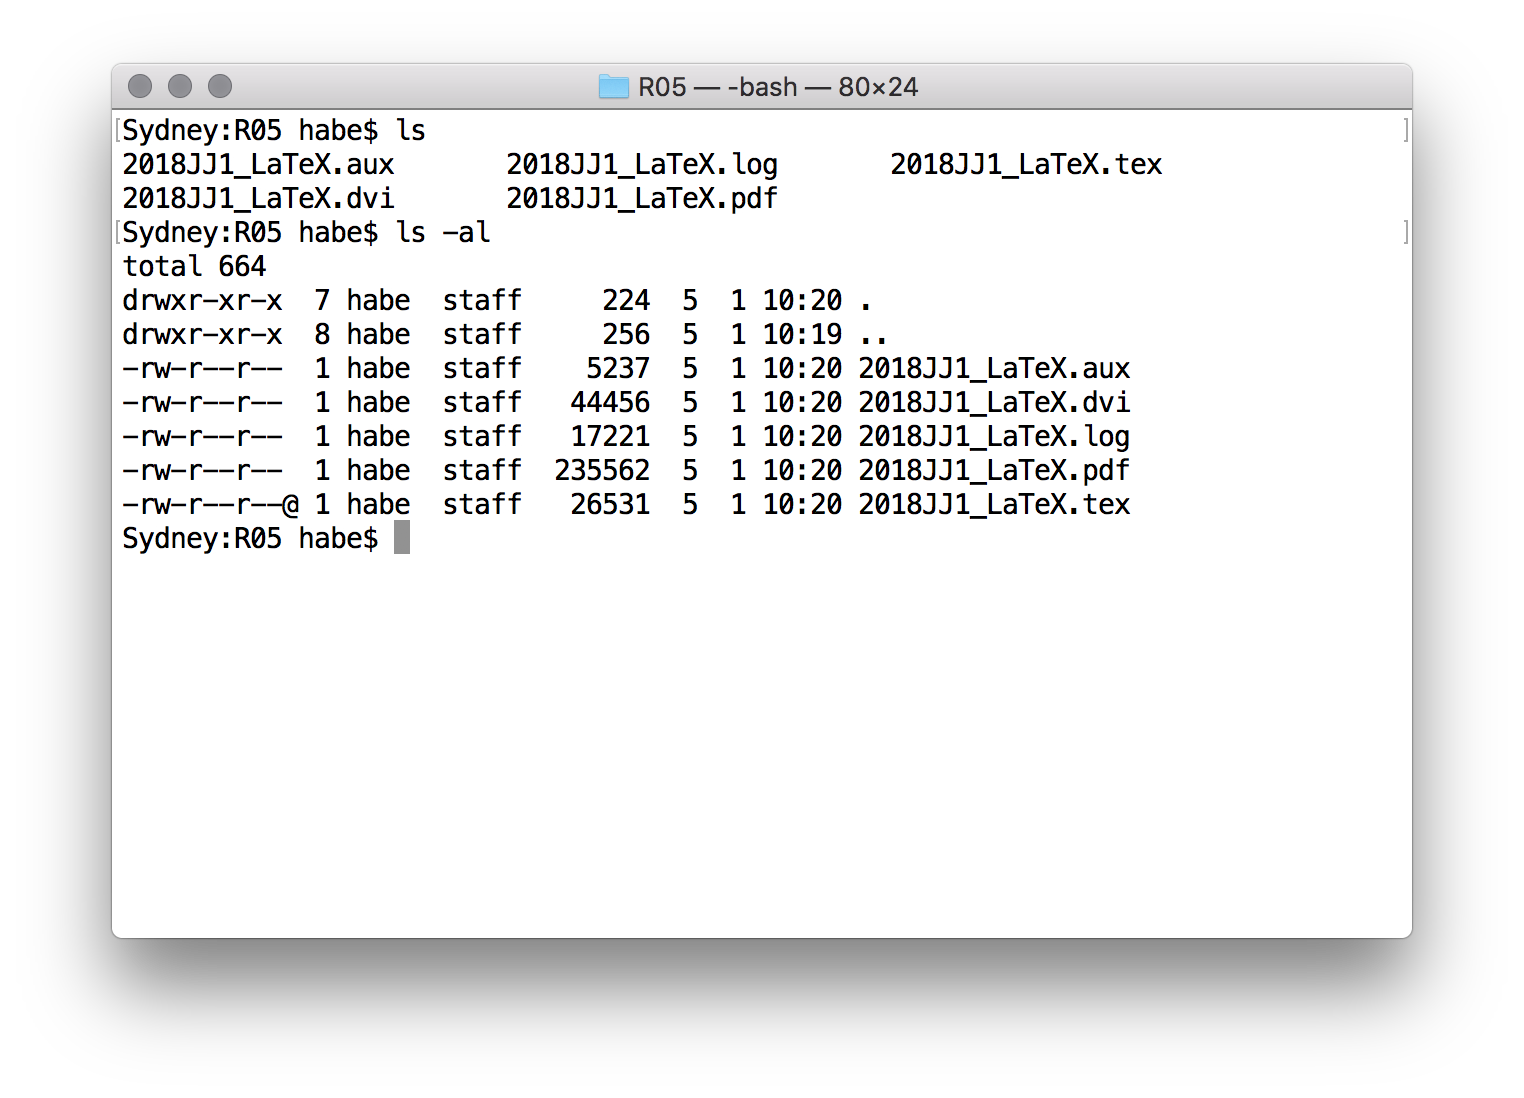
\includegraphics[scale=0.6,clip]{ls.png}
\caption{ls,ls ‐ al コマンド実行の様子}
\label{fig:ls}
\end{center}
\end{figure}
\end{verbatim}
\end{screen}

\begin{figure}[!h]
\begin{center}
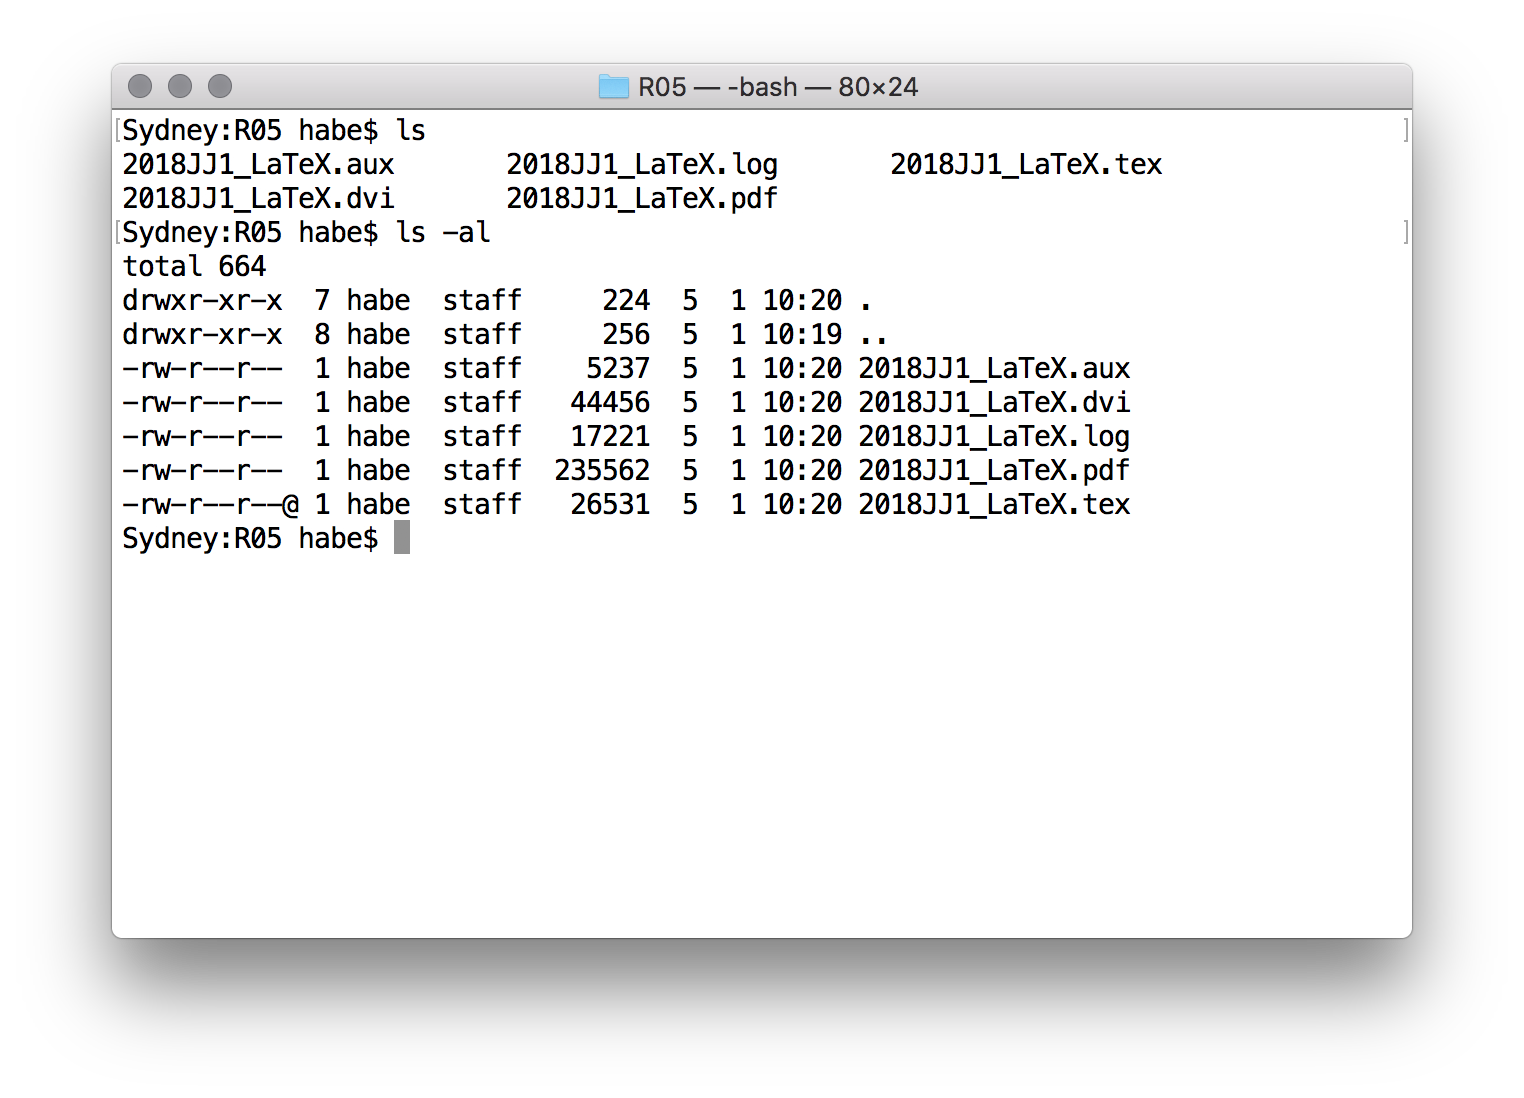
\includegraphics[scale=0.6,clip]{ls.png}
\caption{ls,ls ‐ al コマンド実行の様子}
\label{fig:ls}
\end{center}
\end{figure}

これを順を追って説明していく.
\begin{itemize}
    \item 最初の行の \verb|\begin{figure}| と最後の行の \verb|\end{figure}| の対で \verb|figure| 環境を使ってる.\verb|table| 環境と同じように,図の配置を決め,その中に画像など図の本体や見出しを記述する.

    \item \verb|\begin{figure}| のあとについている \verb|[!h]| は表の配置を指定するオプションである.配置を指定するオプションは表と同じであり,表\ref{table:position}のような種類がある.
    \item \verb|center|環境は\ref{sec:alignment}節で説明したとおり,中央に揃える環境である.
    \item \verb|\includegraphics| が画像を挿入するコマンドである.ここで指定されているオプションの意味は次のとおりである.
    \begin{description}
        \item[] \verb+scale=0.6+:元の画像サイズの0.6倍で出力する.タイプセットしたあとの大きさを確認して適切な数値にすること.小さくて図中の文字が見えないようなことは厳禁である.
        \item[] \verb+clip+:はみ出した分を切り取る.通常は指定しておいた方が良い.
        \item[] \verb+{ls.png}+:\verb+{}+で画像ファイルを指定する.当然ながらファイル名を間違って存在しないものを指すとエラーになるので注意する.なお,ここに相対パスでファイル名を書くと,コマンドを実行したディレクトリからみたものとして解釈される.
    \end{description}
    \item \verb|\caption{}| は図の見出しを指定する.表では見出しは表本体の上部に書き,図では見出しは図本体の下部に書く.
    \item \verb|\label{}| は相互参照を用いるときに使用するラベルを指定する.詳しくは\ref{sec:cross_reference}節で述べている.
\end{itemize}
画像ファイルを準備する方法は様々であるが,実習資料ではスクリーンショットをとる方法を解説している.


\subsection{数式の記述}
\label{sec:math}

\ref{sec:TeXandLaTeX}節で述べたように,数式を簡単に入力できるのが \LaTeX の大きな特長の一つである.最近は,MS Word などでも数式を簡単に入力できるようになっているが,\LaTeX の記法にならっていることが多いので,\LaTeX に習熟していれば様々な場面でも役立つ,

標準でもある程度の数式を記述できるが,\AmS - \LaTeX パッケージ\footnote{アメリカ数学会(American Mathematical Society)向けに開発されたものであるので,数学者向けの機能が備わっている.}には様々な便利な機能が備わっているので,以降では \AmS - \LaTeX を含めて基本的な利用方法を解説していく.まず,\AmS - \LaTeX パッケージを利用するための「おまじない」をプリアンブル(\ref{sec:source}節参照)に
\begin{screen}
\begin{verbatim}
\usepackage{amsmath}
\end{verbatim}
\end{screen}
と記述しておく.

\subsubsection{インライン数式とディスプレイ数式}

\LaTeX で数式を記述する場合には,「インライン数式」と「ディスプレイ数式」の二つの方法がある.

インライン数式とは,文中で数式を扱うための方法であり,
文中で式を \$ で囲むように記述する.
例えば,ソースファイルで \verb|$ax+b$| と書いた場合,
出力結果は $ax+b$ となる\footnote{細かいが  \$ で囲んだ部分の前後には半角スペースを入れた方が見栄えが良い. }.
これに対して,数式モードを使わずに \verb|ax+b| と書いた場合には ax+b となり出力結果が異なっている.
数式モードで出力すると斜体で出力されるが,数式モードを使わない場合はローマン体で出力されるので,
くれぐれも間違えないようにすること.

ディスプレイ数式とは,\verb|equation| や \verb|align| 環境を用いて,
別行立てで数式を記述する方法である.
例として,\verb|align| 環境を用いた数式を以下に記述する.

\begin{screen}
\begin{verbatim}
\begin{align}
f(x) = a x^{2} + b
\end{align}
\end{verbatim}
\end{screen}
このように記述すると,以下のように出力される.
%
\begin{align}
f(x) = a x^{2} + b
\end{align}

この例では,\verb|x^{2}| としている部分は出力例のように \verb|x| の「肩にのせる」ものを指定している.べき乗などを記述する際に用いる.

\subsubsection{verbatim 環境}

数式とは直接関係ないが,\verb|verbatim|環境はソースファイルに記述した内容をそのまま出力する.例えば,
\begin{screen}
\begin{verbatim*}
\begin{verbatim}
\begin{align}
f(x)=ax^{2}+b
\end{align}
\end{verbatim}
\end{verbatim*}
\end{screen}
と記述すれば,
\begin{verbatim}
\begin{align}
f(x)=ax^{2}+b
\end{align}
\end{verbatim}
と表示される.ここでは \LaTeX のソースファイルに記述する内容を示すために用いているが,今後作成するプログラムのソースファイルをレポート中に記載する場合などにも利用できる.また,\verb|verbatim| の代わりに \verb|verbatim*| 環境を用いれば半角スペースを記号に置き換えたものが表示される.ぜひ試してみるとよい.

\subsubsection{数式で用いる文字・記号・演算子}

数式を記述するために必要な文字・記号・演算子を表\ref{tab:math_symbols}にまとめる.記号などは英語での呼び方がコマンドになっている場合が多く,馴染みがないものもあると思うが,必要に応じてマニュアルを参照しながら書いていけば良い.表 \ref{tab:math_symbols} に挙げているのは一部分である.たとえば \cite{Kagishippo} のような Web サイトにも様々なコマンドがまとめられているので,随時参考にすればよい.

\begin{table}[h]
\centering
\caption{数式で用いる文字・記号・演算子}
\label{tab:math_symbols}
\begin{tabular}{ccccc}
\begin{tabular}{c|c}
\multicolumn{2}{c}{ギリシャ文字}  \\
コマンド & 出力 \\ \hline
\verb|\alpha| & $\alpha$ \\
\verb|\beta| & $\beta$ \\
\verb|\gamma| & $\gamma$ \\
\verb|\delta| & $\delta$ \\
\verb|\pi| & $\pi$ \\
\verb|\mu| & $\mu$ \\
\verb|\sigma| & $\sigma$ \\
\verb|\omega| & $\omega$ \\
& \\
&
\end{tabular} & &
\begin{tabular}{c|c}
\multicolumn{2}{c}{関係・二項演算子} \\
コマンド & 出力 \\ \hline
\verb|\times| & $\times$ \\
\verb|\div| & $\div$ \\
\verb|\pm| & $\pm$ \\
\verb|\ne| & $\ne$ \\
\verb|\leq| & $\leq$ \\
\verb|\geq| & $\geq$ \\
\verb|\in| & $\ln$ \\
\verb|\notin| & $\notin$ \\
\verb|\cap| & $\cap$ \\
\verb|\cup| & $\cup$
\end{tabular} & &
\begin{tabular}{c|c}
\multicolumn{2}{c}{三角関数・数学記号} \\
コマンド & 出力 \\ \hline
\verb|\sin| & $\sin$ \\
\verb|\cos| & $\cos$ \\
\verb|\tan| & $\tan$ \\
\verb|\log| & $\log$ \\
\verb|\lim| & $\lim$ \\
\verb|\exp| & $\exp$ \\
\verb|\min| & $\min$ \\
\verb|\max| & $\max$ \\
\verb|\arg| & $\arg$ \\
&
\end{tabular}
\end{tabular}
\end{table}

\subsubsection{行列}

線形代数などでよく扱う行列も \LaTeX を使えば簡単に記述でき,美しく組版できる.\LaTeX 標準の \verb|array| 環境を使っても良いが,ここではより高機能な \verb|pmatrix| 環境を紹介する.

\begin{screen}
\begin{verbatim}
\begin{align}
\begin{pmatrix}
\alpha & \beta
\\
\gamma & \delta
\end{pmatrix}
\end{align}
\end{verbatim}
\end{screen}
このように記述すると,以下のように出力される.
%
\begin{align}
\begin{pmatrix}
\alpha & \beta
\\
\gamma & \delta
\end{pmatrix}
\end{align}

行列の記述方法は\ref{sec:table}節で説明した表の記述方法と似ており,\verb|\\| が改行を示し,\verb|&| が列の区切りを示している.ソースと出力例を照らし合わせて見て欲しい.

もう少し複雑な例としては,

\begin{screen}
\begin{verbatim}
\begin{align}
\begin{pmatrix}
\alpha & \beta
\\
\gamma & \delta
\end{pmatrix}
\begin{pmatrix}
x_{1}
\\
x_{2}
\end{pmatrix}
=
\begin{pmatrix}
\alpha x_{1} + \beta x_{2}
\\
\gamma x_{1} + \delta x_{2}
\end{pmatrix}
\end{align}
\end{verbatim}
\end{screen}

とすれば,

\begin{align}
\begin{pmatrix}
\alpha & \beta
\\
\gamma & \delta
\end{pmatrix}
\begin{pmatrix}
x_{1}
\\
x_{2}
\end{pmatrix}
=
\begin{pmatrix}
\alpha x_{1} + \beta x_{2}
\\
\gamma x_{1} + \delta x_{2}
\end{pmatrix}
\end{align}

のように出力される.\verb|pmatrix| 環境で表現される行列が一つの記号のようになっていることに注意されたい.

\subsubsection{分数・平方根}

これまでに紹介したものの他に,数式では分数や平方根もよく登場する.

\begin{screen}
\begin{verbatim}
\begin{align}
g(x) = \frac{a}{b} x^{2} + \sqrt{c}
\end{align}
\end{verbatim}
\end{screen}
このように記述すると,以下のように出力される.
%
\begin{align}
g(x) = \frac{a}{b} x^{2} + \sqrt{c}
\end{align}

\verb|\frac{a}{b} | は分数を記述するコマンドである.出力例を見ればわかるように \verb|\frac| の次に分子,その次に分母を記述する.\verb|\sqrt{c}|  は平方根を記述するものである.\verb|\frac{a}{b}| と \verb|\sqrt{c}| のどちらも括弧の名に記述した数式が大きくなってもバランスよく数式が配置されるように自動調整される.

\subsection{参考文献リスト}

レポートや論文などを書くときには,まったく何も参考にせずに,ゼロから書き上げることはまず起こりえない.必ず何らかのを文献を参考にし,そこから得た知識を利用して,自らの考察・提案をまとめていくことになる.どの部分を参考にし,どの部分が独創的な部分なのかを明確にするためにも,参考文献リストを明示し,それが本文のどの部分に関与しているのかを明らかにしておく必要がある.

参考文献リストを作成するために,\LaTeX には様々な便利な機能が備わっているが,ここではもっとも単純なものを紹介しておく\footnote{\BibTeX というツールを使えば,あらかじめ用意しておた文献データベースから自動的に整形して参考文献リストを作成できる.} .

参考文献リストは文章の末尾に以下のように記述しておく.
\begin{screen}
\begin{verbatim}
\begin{thebibliography}{9}
   \bibitem{TeXText} 渡辺徹,好き好き \LaTeXe 初級編,2006.
   \bibitem{Kagishippo} 「物理のかぎしっぽ」\TeX に関するメモ,2021年5月17日閲覧.
\end{thebibliography}
\end{verbatim}
\end{screen}
この例は本書の末尾にある参考文献リストとほぼ同じもの出力するためのソースである\footnote{Webアドレスを書くと長くなるので省略している.}.簡単にその内容を説明する.
\begin{itemize}
\item \verb|\begin{thebibliography}| のあとにある \verb|{9}| の数値は参考文献数の桁数を示している.もし参考文献の数が一桁であれば 9 ,二桁であれば 99 のように記述する.
\item \verb|\bibitem| で始まる項目がそれぞれの参考文献を指している.\verb|\bibitem| は直後に参照キーを指定する.本文ではこの参照キーを使って参考文献を指し示す.
\end{itemize}
このような参考文献リストを用意したあとで,本文中では \verb|\cite| コマンドを使って参考文献について言及する.たとえば,
\begin{screen}
\begin{verbatim}
情報実習Iでは教科書\cite{TeXText}を指定しているが,教科書は非常に細かに記述されているので,いきなり教科書を読んでも理解は難しいかもしれない.
\end{verbatim}
\end{screen}
とソースファイルに書けば,
\begin{screen}
情報実習Iでは教科書\cite{TeXText}を指定しているが,教科書は非常に細かに記述されているので,いきなり教科書を読んでも理解は難しいかもしれない.
\end{screen}
と出力される.参照キーを用いれば,それが何番の参考文献に相当するかは \LaTeX が自動的に判断して番号に置換される.

なお,参考文献リストでWebページのアドバイスを示すときには \verb+ url + パッケージを使えば便利である.プリアンブルに
\begin{screen}
\begin{verbatim}
\usepackage{url}
\end{verbatim}
\end{screen}
と書いておけば,
\begin{screen}
\begin{verbatim}
\url{https://www.kindai.ac.jp/science-engineering/}
\end{verbatim}
\end{screen}
という命令をソースファイルに書けば,
\begin{screen}
\url{https://www.kindai.ac.jp/science-engineering/}
\end{screen}
のようにリンク付きで表記される.なお,\verb+ url + 命令の中にアドレスを書くときには,中に \verb+ _ + などの特殊文字があっても問題ない.

   

\begin{thebibliography}{1}
   \bibitem{TeXText} 渡辺徹,好き好き \LaTeXe 初級編,\url{https://mytexpert.osdn.jp/index.php?%B9%A5%A4%AD%B9%A5%A4%ADLaTeX2e/%BD%E9%B5%E9%CA%D4},2006.
   %\bibitem{JJ1-3} 情報実習I解説スライド(第3回),近畿大学理工学部情報学科,2019.
   %\bibitem{JJ1-5} 情報実習I解説スライド(第5回),近畿大学理工学部情報学科,2019.
   \bibitem{Kagishippo} 「物理のかぎしっぽ」\TeX に関するメモ,\url{http://hooktail.org/computer/index.php?TeX},2020年5月27日閲覧.
\end{thebibliography}

\begin{flushright}
以上
\end{flushright}

\end{document}
